\documentclass{beamer}



\usepackage[utf8]{inputenc}
\usepackage[ngerman]{babel}
\usepackage{verbatim}
\usepackage{hyperref}
\usepackage{url}
\usepackage{fancyvrb}

\title{Anwendung von freien Geodaten auf mobilen Navigationsgeräten}
\author{Stefan Tiran  stefan.tiran@student.TUGraz.at}
\date{April 25th, 2013}

\usetheme{Antibes}

%\usebackgroundtemplatei{
%\includegraphics[width=\paperwidth,
%height=0.8\paperheight]{mag_map.png}
%}

\begin{document}

%\maketitle

\begin{frame}


\begin{figure}
  \centering
  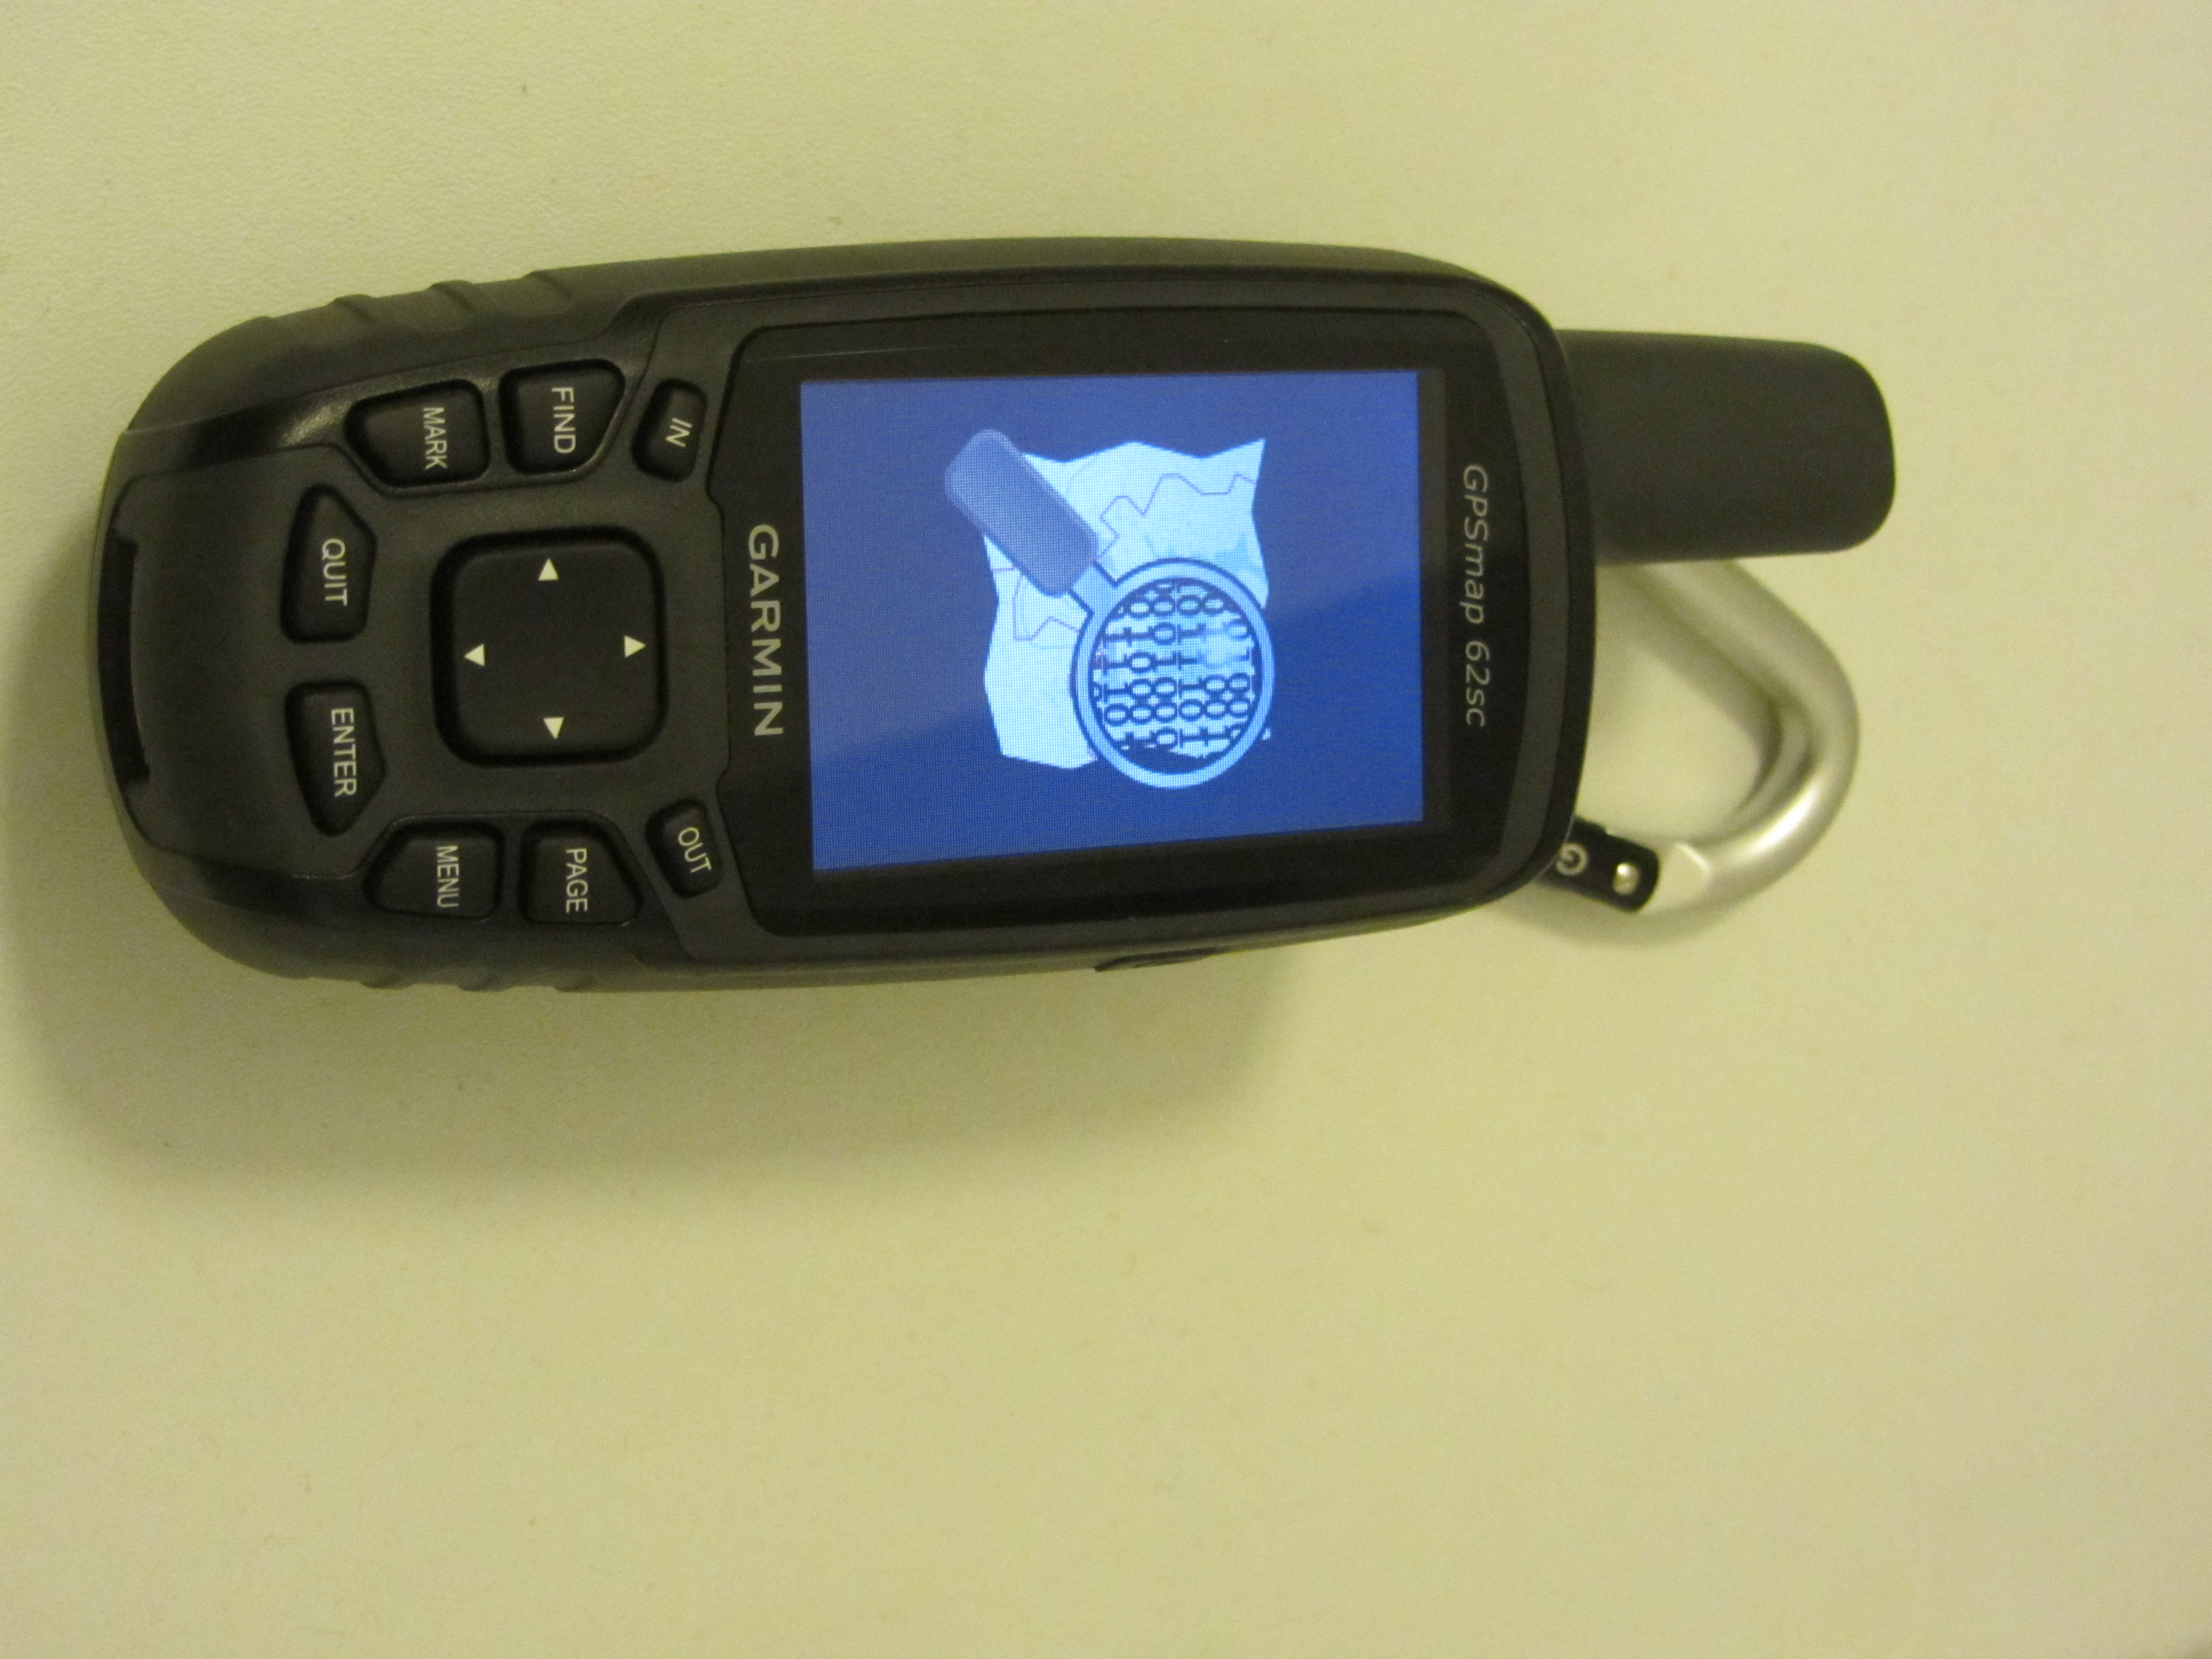
\includegraphics[angle=90,width=.3\textwidth]{IMG_6589.JPG}
\end{figure}

\begin{center}
\Large{Anwendung von freien Geodaten auf mobilen Navigationsgeräten\\}
\end{center}

\begin{center}
{\emph{Freie Karten, Routen und POIs auf herkömmlichen Navigationsgeräten verwenden}}
\end{center}
\end{frame}

\begin{frame}{Über den Vortragenden}

  \begin{itemize}
    \item Stefan Tiran \textless \href{mailto:stefan.tiran@student.TUGraz.at}{stefan.tiran@student.TUGraz.at}\textgreater
    \item Diplomand (Softwareentwicklung-Wirtschaft) an der TU Graz
    \item Linux-User (SuSE / Ubuntu) seit 2003
    \item OpenStreetMap seit August 2008
    \begin{itemize}
      \item OSM-Username: \emph{StefanTiran}
      \item Mapping-Area Graz, Südsteiermark
      \item Mit Fahrrad und Öffis
    \end{itemize}
  \end{itemize}
\end{frame}

\section{Datenquellen}
\subsection{OpenStreetMap}
\begin{frame}{OpenStreetMap}
  \begin{itemize}
    \item Freie Weltkarte nach dem Wiki-Prinzip
    \item \url{http://www.openstreetmap.de/}
    \item Lizenz: ODbL
    \item Bietet an:
    \begin{itemize}
      \item Karten (Straßen, Wege, Flüße, Skipisten,...)
      \item Points Of Interest (Lokale, Geschäfte,
        Sehenswürdigkeiten,...)
      \item Routen (Buslinien, Radwege,...)
    \end{itemize}
  \end{itemize}
\end{frame}
\subsection{UMP-pcPL}
\begin{frame}{UMP-pcPL}
  \begin{itemize}
    \item Unofficial Map of Poland
    \item \url{http://ump.waw.pl/en/}
    \item Freie Europa-Karte mit Fokus Polen und Osteuropa
    \item Zugeschnitten auf Garmin-Geräte
    \item Initiiert: 2002
    \item Lizenz: CC BY-SA 3.0
    \item Bietet an:
    \begin{itemize}
      \item Karten
      \item POIs in Karte integriert
    \end{itemize}
  \end{itemize}
\end{frame}

\subsection{OGD}
\begin{frame}{OGD}
  \begin{itemize}
    \item Open Government Data Initiativen der Gebietskörperschaften
      Österreichs
    \item \url{http://data.gv.at/} -- offene Daten Österreichs
    \item Städte: Wien, Linz, Graz
    \item Bundesländer: Steiermark, Niederösterreich, Tirol,
      Vorarlberg, Oberösterreich
    \item Lizenz: Unterschiedlich; meist CC BY-SA
    \item Bieten an: (mit Geobezug, Auszug)
    \begin{itemize}
      \item ``Basiskarte Graz mit Hausnummern'' als Bitmap
      \item POIs (Apotheken, Ärzte, Schulen,...)
      \item Radwege, Flüsse, Seen, Teiche, Hochrangiges Straßennetz
    \end{itemize}
    \item Eher Quelle für OpenStreetMap als Direktverwendung der Daten
  \end{itemize}
\end{frame}

\section{Geräte}
\begin{frame}
  \begin{itemize}
    \item Garmin: Proprietäres Format, aber gut
      verstanden
    \item Magellan: Proprietäres Format, teilweise
      verstanden, kommerzielles SDK
    \item Android: Verschiedene Software (frei und proprietär)
    \item Windows Mobile: Verschieden Software (frei und proprietär)
  \end{itemize}
\end{frame}

\subsection{Garmin - vorgefertigte Karten}
\begin{frame}
Garmin - vorgefertigte Karten
\begin{itemize}
  \item Große Auswahl an vorgefertigten Karten
  \item \url{http://wiki.openstreetmap.org/wiki/Garmin-Maps}
  \item nicht alle sind routingfähig
  \item Adresseingabe teilweise unausgereift; besser POIs verwenden
  \item unterschiedliche Länder
  \item unterschiedliche Einsatzgebiete (Fahrrad, Auto, Reit- und
    Wanderkarte)
  \item \texttt{gmapsupp.img} oder einzelne Kacheln
  \item Größenlimitierungen des Gerätes beachten (2 GB, 4, GB, mehrere
    Dateien möglich?)
  \item Kartentankstelle am OSM-Stand!
\end{itemize}
\end{frame}

\subsection{Garmin - selbstgemachte Karten}
\begin{frame}
  Garmin - selbstgemachte Karten
  \begin{itemize}
    \item Wiki hilft:
      \url{http://wiki.openstreetmap.org/wiki/DE:OSM_Map_On_Garmin}
    \item Programme:
    \begin{itemize}
      \item \texttt{mkgmap} Kommandozeile
      \item \texttt{mkgmapgui} GUI
    \end{itemize}
    \item Ablauf: \texttt{.osm}-Datei exportieren und umwandeln
    \item Schnell für sehr kleine Ausschnitte
    \item Ansonsten: Vorverarbeitung erforderlich
  \end{itemize}
\end{frame}

\section{Herstellerunabhängig}
\subsection{GPX}
\begin{frame}
  GPX
  \begin{itemize}
    \item GPS Exchange Format
    \item Unterstützt Wegpunkte, Routen und Tracks
    \item Umwandlung zwischen \texttt{.osm} und \texttt{.gpx}:
    \begin{itemize}
      \item \texttt{osmconvert} Kommandozeile, Vorverarbeitung \footnote{\url{http://wiki.openstreetmap.org/wiki/DE:Osmconvert}}
      \item \texttt{gpsbabel} Kommandozeile, viele Optionen, viele Formate
      \item JOSM: eigentlich Editor; GUI
    \end{itemize}
  \item Teilweise Webservices
  \end{itemize}
\end{frame}

\subsection{Fallbeispiel 1: Sulmtalradweg}
\begin{frame}
Fallbeispiel 1: Sulmtalradweg
\begin{itemize}
  \item
    % \url{http://wiki.openstreetmap.org/wiki/WikiProject_Austria/Radwege}%
\url{http://wiki.openstreetmap.org/wiki/WikiProject_Austria/Radwege\#Radwege_in_der_Steiermark}
\end{itemize}
  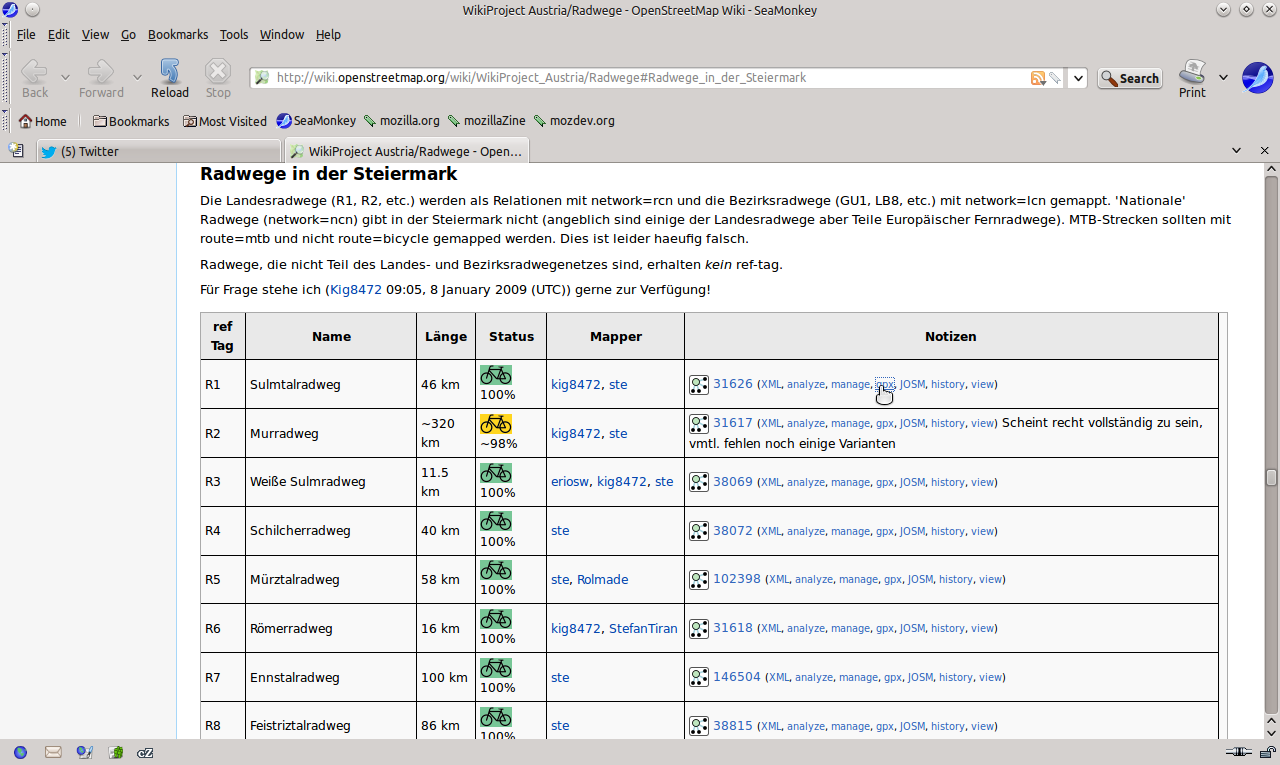
\includegraphics[width=\textwidth, trim=150 100 50 100,clip]{cs1.png}

\end{frame}

\subsection{Fallbeispiel 2: Nichtraucherlokale in Graz}
\begin{frame}[fragile]
%\newcommand\vitem[1][]{\SaveVerb[%
%    aftersave={\item[\textnormal{\UseVerb[#1]{vsave}}]}]{vsave}}

%  \begin{itemize}
%    \item XAPI
\verb+#!/bin/bash+
\verb+#Schritt 1: OSM-Datenbank abfragen via XAPI+
\verb+wget "http://overpass-api.de/api/xapi?*[smoking=no]\+
\verb+[amenity=restaurant|cafe]\+
\verb+[bbox=15.34,47,15.55,47.15][@meta]" \+
\verb+-O graz_smoking_no.osm+
\\
\verb+#Schritt 2: Wege und Relationen in Punkte umwandeln+
\verb+osmconvert --all-to-nodes graz_smoking_no.osm \+
\verb+           -o=graz_smoking_no_nodes.osm+
\end{frame}
\begin{frame}[fragile]


\verb+#Schritt 3: In GPX umwandeln +

\verb+gpsbabel -i osm -f graz_smoking_no_nodes.osm \+
\verb+         -o gpx -F graz_smoking_no.gpx+
\\
\verb+#Schritt 4: Symbole vereinheitlichen (optional)+
\verb+sed -i 's|<sym>.*</sym>||g' graz_smoking_no.gpx+
\verb+sed -i 's|</wpt>|<sym>Navaid, Red</sym>\+
\verb+</wpt>|g' graz_smoking_no.gpx+
%\end{Verbatim}
%    \item x
%  \end{itemize}
\end{frame}

\end{document}


%%:foldmethod=expr
%% vim:fde=getline(v\:lnum)=~'^%%%%\ .\\+'?'>1'\:'='
%%% Local Variables: 
%%% mode: latex
%%% mode: auto-fill
%%% mode: flyspell
%%% eval: (ispell-change-dictionary "de_AT")
%%% TeX-master: "main"
%%% End: 

